\documentclass[10pt,twocolumn,letterpaper]{article}

\usepackage{cvpr}
\usepackage{times}
\usepackage{epsfig}
\usepackage{graphicx}
\usepackage{amsmath}
\usepackage{amssymb}
\usepackage{caption}
\usepackage{subcaption}
\usepackage{tikz}
\usetikzlibrary{fit,positioning,calc}

% Include other packages here, before hyperref.

% If you comment hyperref and then uncomment it, you should delete
% egpaper.aux before re-running latex.  (Or just hit 'q' on the first latex
% run, let it finish, and you should be clear).
\usepackage[breaklinks=true,bookmarks=false]{hyperref}

\cvprfinalcopy % *** Uncomment this line for the final submission

\def\cvprPaperID{****} % *** Enter the CVPR Paper ID here
\def\httilde{\mbox{\tt\raisebox{-.5ex}{\symbol{126}}}}

% Pages are numbered in submission mode, and unnumbered in camera-ready
%\ifcvprfinal\pagestyle{empty}\fi
\setcounter{page}{1}
\begin{document}

%%%%%%%%% TITLE
\title{Articulated Motion Models for Scene Understanding}

\author{Suren Kumar\\
SUNY Buffalo \\
Buffalo, NY \\
{\tt\small surenkum@buffalo.edu}
% For a paper whose authors are all at the same institution,
% omit the following lines up until the closing ``}''.
% Additional authors and addresses can be added with ``\and'',
% just like the second author.
% To save space, use either the email address or home page, not both
\and
Vikas Dhiman, Jason J. Corso\\
University of Michigan\\
Ann Arbor, MI\\
{\tt\small \{dhiman@,jjcorso@eecs\}.umich.edu}
\and
Venkat N. Krovi\\
SUNY Buffalo \\
Buffalo, NY \\
{\tt\small vkrovi@buffalo.edu}}

\maketitle
%\thispagestyle{empty}

%%%%%%%%% ABSTRACT
\begin{abstract}
We hypothesize a articulated model world view of scene understanding by representing scene as collection of objects/bodies (humans, chairs, doors, walls, floor etc.) which are connected to each other by various types of articulated joints (prismatic, revolute, static, motion along a plane etc.). Spatial structure of scene is due to the nature of these articulated joints, i.e. objects do not exhibit motions with full degree of freedom (6 for 3-dimensional world) but instead have a structure afforded by the articulated joint (door moves about a hinge). Along with this spatial structure, we hypothesize motion in world is temporally structured by finite order of motion. We use this spatio-temporal structure to represent the scene and demonstrate the proposed framework for the problem of Simultaneous localization and Area Mapping in dynamic environments.
\end{abstract}

%%%%%%%%% BODY TEXT
\section{Introduction}

Imagine a robot moving in a typical living room environment which encounters indoor objects such as doors, drawers and chairs etc. We posit that in order for the robot to understand, map or interact with such objects, the robot needs to be able to understand the articulation. 
%Pyschophysical experiments on human motion understanding have demonstrated that human first distinguish between competing motion models (translation, rotation and expansion) and then estimate the motion conditioned on motion model \cite{NIPS2008_3458}. 

%-------------------------------------------------------------------------
\section{Motion Models in Literature}
There is significant interest in modelling motion for object tracking in computer vision literature \cite{cifuentes2012motion}. However the modelling of motion is often done in image space with simplistic models such as move left/move right which does not explain the motion of objects in physical world. Yan and Pollefeys \cite{yan2006automatic} proposed a model to detect the articulated structure of a object by using Structure from motion and then clustering trajectories to find articulation. But their approach only models revolute joint and doesn't model the temporal structure. 

There has been tremendous interest in robotics community to learn the kinematic structure such as the type of articulation from depth data \cite{katz2014interactive}. However the primary limitation of such methods is the restricted work space as they do not model the appearance/dis-appearance of objects from the scene because they do not make any map of the world.

SLAM deals with dynamic environment in two different ways, 1) State Augmentation \cite{wang2003online,kundu2011realtime} which adds the state of the moving objects to the overall state being estimated, 2) Outlier Rejection which aims to detect and remove the objects/landmarks from the mapping and localization estimation. However, both these approaches fail to model the motion of moving features/landmarks in a robust manner which precludes the possibility of using moving landmarks for both localization and mapping. 
% State augmentation approach  \cite{wang2003online}. State augmentation approaches \cite{wang2003online,kundu2011realtime} assume the separation of measurement into stationary and moving objects and map is still built from static features.  On the other hand outlier rejection aims to detect and remove the objects/landmarks from the mapping and localization estimation. However, both these approaches fail to model the motion of moving features/landmarks in a robust manner which precludes the possibility of using moving landmarks for both localization and mapping.  The generic and common method used to model the motion is that of constant velocity model in 3D euclidean coordinates \cite{wang2003online}, Special Euclidean group SE(3) of transformation \cite{kundu2011realtime}. This velocity model is insufficient to model the physical reality such as motion of a door, movement of a chair on the floor etc.

The proposed approach uses robust and physically inspired models of spatio-temporal motion which can be used to accurately describe the motion and hence enabling moving landmarks to be used in localization and mapping.


\begin{figure*}[t]
  \begin{subfigure}[t]{0.33\textwidth}
    \scalebox{0.65}{ 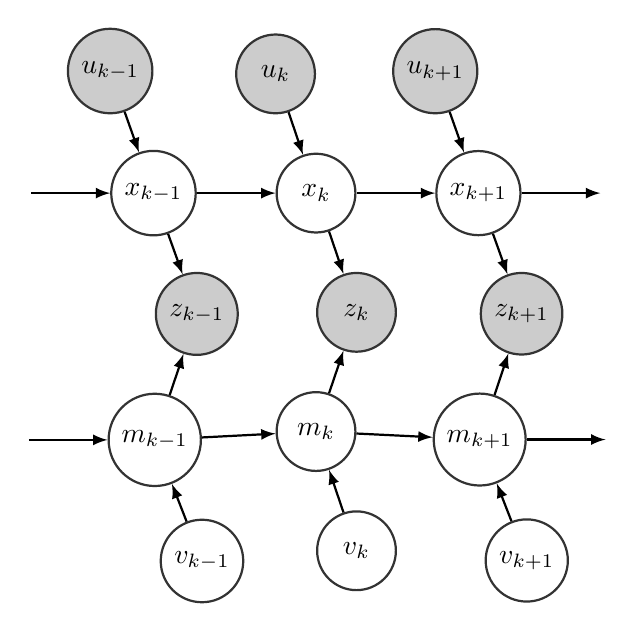
\begin{tikzpicture}
\tikzstyle{main}=[circle, minimum size = 10mm, thick, draw =black!80, node distance = 10mm]
\tikzstyle{connect}=[-latex, thick]
\tikzstyle{box}=[rectangle, draw=black!100]
\coordinate (org_1) at (0,0);
  \node[main] (x_k_1)[right=of org_1] {$x_{k-1}$ };
  \node[main] (x_k) [right=of x_k_1] { $x_{k}$ };
  \node[main] (x_k_2) [right=of x_k] {$x_{k+1}$};
\coordinate[right=of x_k_2] (end_1);

  \node[main, fill = black!20] (u_k_1)[above=of x_k_1.west] {$u_{k-1}$ };
\node[main, fill = black!20] (u_k)[above=of x_k.west] {$u_{k}$ };
\node[main, fill = black!20] (u_k_2)[above=of x_k_2.west] {$u_{k+1}$ };

\node[main, fill = black!20] (z_k_1)[below=of x_k_1.east] {$z_{k-1}$ };
\node[main, fill = black!20] (z_k)[below=of x_k.east] {$z_{k}$ };
\node[main, fill = black!20] (z_k_2)[below=of x_k_2.east] {$z_{k+1}$ };


\node[main] (m_k_1)[below=of z_k_1.west] {$m_{k-1}$ };
\coordinate [left=of m_k_1](org_2);
\node[main] (m_k)[below=of z_k.west] {$m_{k}$ };
\node[main] (m_k_2)[below=of z_k_2.west] {$m_{k+1}$ };
\coordinate [right=of m_k_2](end_2);

\node[main] (v_k_1)[below=of m_k_1.east] {$v_{k-1}$ };
\node[main] (v_k)[below=of m_k.east] {$v_{k}$ };
\node[main] (v_k_2)[below=of m_k_2.east] {$v_{k+1}$ };


  \path 
 (org_1) edge [connect] (x_k_1)
(x_k_1) edge [connect] (x_k)
(x_k) edge [connect] (x_k_2)
(x_k_2) edge [connect] (end_1)

(u_k_1) edge [connect] (x_k_1)
(u_k) edge [connect] (x_k)
(u_k_2) edge [connect] (x_k_2)

(x_k_1) edge [connect] (z_k_1)
(x_k) edge [connect] (z_k)
(x_k_2) edge [connect] (z_k_2)

(m_k_1) edge [connect] (z_k_1)
(m_k) edge [connect] (z_k)
(m_k_2) edge [connect] (z_k_2)


 (org_2) edge [connect] (m_k_1)
(m_k_1) edge [connect] (m_k)
(m_k) edge [connect] (m_k_2)
(m_k_2) edge [connect] (end_2)

(v_k_1) edge [connect] (m_k_1)
(v_k) edge [connect] (m_k)
(v_k_2) edge [connect] (m_k_2);
\end{tikzpicture}
 }
    \caption{Graphical Model of the general SLAM problem. The known nodes are darker than the unknown nodes.}
    \label{fig:graphical_model}
  \end{subfigure}
  \hskip1pt
  \vrule
  \hskip1pt
  \begin{subfigure}[t]{0.67\textwidth}
    \newlength{\imgwidth}
    \setlength{\imgwidth}{0.9\textwidth}
    \centering
     \begin{tikzpicture}[imgstyle/.style={draw,thick,anchor=south west,inner sep=1pt}]
   %\path[use as bounding box, draw] (0,0) rectangle (\textwidth, 7);
\node[imgstyle] (img1) at (0,0) {\includegraphics[width=0.32\textwidth]{media/frame0000.png}};
\node[imgstyle] (img2) at (0.333\textwidth,0) {\includegraphics[width=0.32\textwidth]
{media/frame0003.png}};
\node[imgstyle] (img3) at (0.666\textwidth,0) {\includegraphics[width=0.32\textwidth]{media/frame0009.png}};
\begin{scope}[x={(img1.south east)}, y={(img1.north west)}]
\node (r) at (0.3, 0.1) {Robot};
\node (lmks) at (0.7, 0.6) {Landmarks};
\end{scope}
\path ($(img1.south) + (1, -0.5)$) node (ld) {Legend:};
\path 
(ld)
 ++ (1.8, 0) node [circle,fill=green] {} + (1, 0) node {Prismatic}
 ++ (3, 0) node [circle,fill=blue] {} + (1, 0) node {Revolute}
 ++ (3, 0) node [circle,fill=red] {} + (0.8, 0) node {Static}
;

 \end{tikzpicture}

    \caption{Frames at different time intervals of our simulation.
      Color of a landmark at a particular frame is the weighted sum of colors
      assigned to each motion model. The weights used are the probability of the
    landmark following that particular motion model and estimated by our algorithm. We also show the predicted trajectory of a landmark according to the estimated motion model.}
    \label{fig:results}
  \end{subfigure}
  \caption{Model and Results}
\end{figure*}

\section{SLAM for Dynamic World}
\begin{figure}

\end{figure}
Figure \ref{fig:graphical_model} shows the graphical model of the most general SLAM problem, where $x_k$, $u_k$, $z_k$, $m_k$, $v_k$ represents the robot state, input to the robot, observation by robot, state of the world and action of various agents in the environment.

% Basic SLAM algorithms \textit{assume the map $m_{k-1} \equiv m_k \equiv m$ to be static} and model the combination of robot state and map $x_k,m$ as the state of the estimation problem. The estimation problem only requires motion model $P(x_k|x_{k-1},u_k)$ and observation model $P(z_k|x_k,m)$. The observation model assumes the observations to be conditionally independent given the the map and the current vehicle state. The goal of the estimation process is to produce unbiased and consistent estimates (expectation of mean squared error should match filter-calculated covariance) \cite{yaakov2001estimation}.

% For the current SLAM problem, the state consists of time-varying map, (unknown input to the world by various agents) and the robot state. Hence the full estimation problem can be posed as 
% \begin{align}
% P(x_k,m_k|\mathbf{Z}_{0:k},\mathbf{U}_{0:k},\mathbf{V}_{0:k},x_0,m_0)
% \end{align}
% Following the notation in the review paper on SLAM by Durrant-Whyte and Bailey \cite{durrant2006simultaneous}, $\mathbf{Z}_{0:k}$, $\mathbf{U}_{0:k}$ and $\mathbf{V}_{0:k}$ represent the set of observations, robot control inputs and map control inputs from the start time to time step $k$. It is assumed that the map is markovian in nature which implies that the start state of the map $m_0$ has all the information needed to make future prediction if actions of various agents in the world $v_{k-1},...,v_{k+1}$ and its impact on the map is known.
% 
\subsection{Time update} The time update models the evolution of state according to the motion model. To write equation concisely, let $A =\{ \mathbf{Z}_{0:k-1},\mathbf{U}_{0:k},\mathbf{V}_{0:k},x_0,m_0 \}$
\begin{multline}
P(x_k,m_k|A) = 
% &\int \int P(x_k,x_{k-1},m_k,m_{k-1}|A) dx_{k-1} dm_{k-1} \nonumber \\
% &\int \int P(x_k|x_{k-1},m_k,m_{k-1},A)P(x_{k-1},m_k,m_{k-1}|A) dx_{k-1}dm_{k-1} \nonumber \\
% &\int \int P(x_k|x_{k-1},u_k)P(x_{k-1},m_k,m_{k-1}|A) dx_{k-1}dm_{k-1} \nonumber \\
% &\int \int P(x_k|x_{k-1},u_k)P(m_k|x_{k-1},m_{k-1},A)P(x_{k-1},m_{k-1}|A)  dx_{k-1}dm_{k-1} \nonumber \\
\int \int P(x_k|x_{k-1},u_k)P(m_k|m_{k-1},v_{k-1})\\P(x_{k-1},m_{k-1}|A) dx_{k-1}dm_{k-1}
\label{eq:time_update}
\end{multline}

The independence relationship in derivation of time update in Equation \ref{eq:time_update} are due to the Bayesian networks in Figure \ref{fig:graphical_model} in which each node is independent of its non-descendants given the parents of that node. Given the structure of time update, we need two motion models, one for robot: $P(x_k|x_{k-1},u_k)$ and another one for the world $P(m_k|m_{k-1},v_{k-1})$. It can be clearly observed that $P(m_k|m_{k-1},v_{k-1})$ for a static map is dirac delta function and integrates out in Equation \ref{eq:time_update}. 
% 
\subsection{Measurement Update} Measurement update uses the bayes formula to update the state of the estimation problem given a new observation $z_k$ at time step $k$. To write the equations concisely, let $B =\{ \mathbf{Z}_{0:k},\mathbf{U}_{0:k},\mathbf{V}_{0:k},x_0,m_0 \}$
 \begin{align}
P(x_k,m_k|B) %&= \frac{P(z_k|x_k,m_k,A)P(x_k,m_k|A)}{P(z_k|A)} \nonumber\\
&=\frac{P(z_k|x_k,m_k)P(x_k,m_k|A)}{P(z_k|A)}
\label{eq:measurement_update}
\end{align}

Equation \ref{eq:measurement_update} together with equation \ref{eq:time_update} defines the complete recursive form of the SLAM algorithm for a dynamic environment. 
%Robot motion model and observation model $P(z_k|x_k,m_k)$ are well described in previous literature and hence we will exclude that from current discussion. The focus of current work is the representation of map motion model to extend the standard SLAM algorithm with its static world assumption to dynamic world.

\section{Dynamic World Representation} 
% Real world is dynamic in nature with varying degree of motion such as parking lot which can be assumed to be temporary stationary compared to a road which is always in motion. Previous literature to handle dynamic environments can be divided into two predominant approaches A) Detect moving objects and ignore them, B) Track moving objects as landmarks  \cite{bailey2006simultaneous}. In the first approach, using the fact that the conventional SLAM map is highly redundant, the moving landmarks can be removed from the map building process \cite{bailey2002mobile}. In contrast, Wang et. al \cite{wang2003online} explicitly track moving objects by adding them to the estimation state. However the work assumed that the sensor measurement can be decomposed into observation corresponding to moving and static landmarks which requires good estimate of moving and static landmarks to start with. Furthermore, it was assumed that the measurement of moving object carries no information for the SLAM state estimation implying that the map remains unchanged. A simple counter example is the case of a moving door in an indoor environment which changes the map of the scene.
% 
% \subsection{Known Decomposition of the World} Object SLAM+ Object Tracking Interacting multiple models
% 
% In feature based mapping, motion of each feature can be assumed to be independent given the location of the feature at previous time step. In dense mapping, a scene/map be decomposed into $n$ different parts such as chair, door etc. whose shape is known. The parts of the scene $m_k = \{b^i_k\},  1\leq i \leq n$ are assumed to move independently and hence the motion of the map can be represented as collection of independent motion of the parts. The true motion model for the  each part of the scene is assumed to be one of the motion models $C \in \{C_j\}^{p}_{j=1}$ as represented in Section \ref{sec:articulation_classification}. 
% 
Dropping the notation for scene part, In current formulation, we assume a uniform prior $\mu_j(0) = P(C_j), \sum_{j=1}^{p}\mu_j(0) = 1$ over different motion models for each scene part. However, this prior can be modified appropriately by object detection such as doors are more likely to have revolute joints etc.. Motion model probability is updated as more and more observations are received \cite{yaakov2001estimation} as 
\begin{align*}
& \mu_j(k) \equiv P(C_j|\mathbf{Z}_{0:k})  = 
%\frac{P(z_k|\mathbf{Z}_{0:k-1}, C_j)P(C_j|\mathbf{Z}_{0:k-1})}{P(z_k|\mathbf{Z}_{0:k-1})} \nonumber \\
%&\mu_j(k) = 
  \frac{P(z_k|\mathbf{Z}_{0:k-1}, C_j)\mu_j(k-1)}{\sum_{j=1}^{p} P(z_k|\mathbf{Z}_{0:k-1}, C_j)\mu_j(k-1) }
\end{align*}
The probability of the current observation $z_k$ at time step $k$, conditioned over a specific motion model and all the previous observation can be represented by various method. In the current work, we filter the states using Extended Kalman Filter, for which this probability is the probability of observation residual w.r.t a normal distribution distributed with zero mean and innovation covariance \cite{yaakov2001estimation}.


\section{Preliminary experiment and Results}
We test our algorithm in a simulated environment of 3 landmarks generated with each of the first order motion models: static, prismatic and revolute. We assume that robot egomotion is known and we use bearing and distance observations from the robot to estimate different motion models over time. 
%In Figure~\ref{fig:results}, the trajectories are drawn when a particular motion model has probability above a threshold.
Our experimental results in Figure~\ref{fig:results}, show that our EKF based motion model and parameter estimation works as expected.

{\small
\bibliographystyle{ieee}
\bibliography{articulation_scene_understanding}
}

\end{document}
